\documentclass[border=5pt]{standalone}
\usepackage[dvipsnames]{xcolor}
\usepackage{tikz}
\usepackage{pgfplots}
\pgfplotsset{compat=1.18}

\definecolor{pwmBlue}{HTML}{2E5FA1}
\definecolor{pwmOrange}{HTML}{E8712B}
\definecolor{pwmGreen}{HTML}{3D9E3F}
\definecolor{pwmRed}{HTML}{C93C3C}

\begin{document}
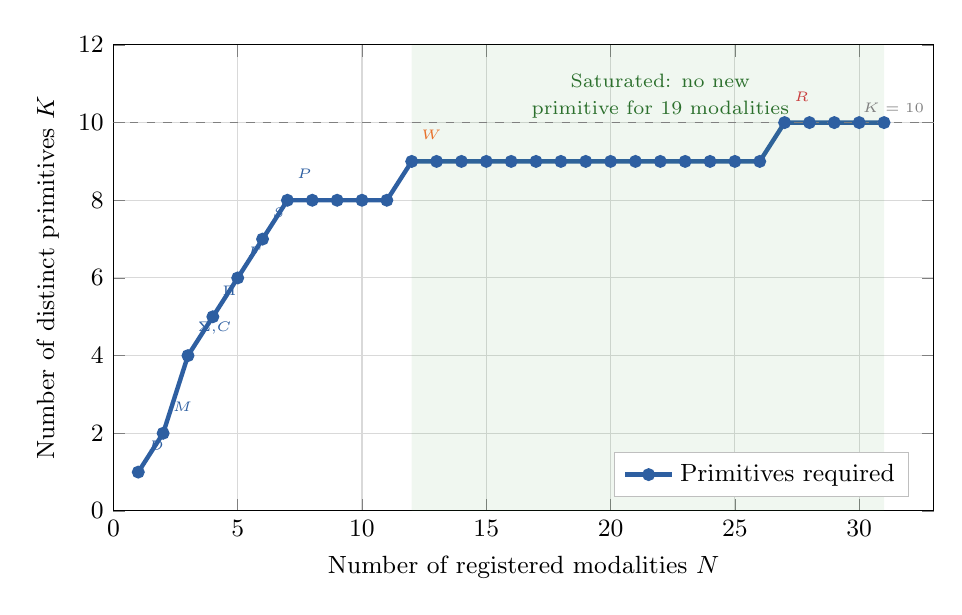
\begin{tikzpicture}
\begin{axis}[
    width=12cm, height=7.5cm,
    xlabel={Number of registered modalities $N$},
    ylabel={Number of distinct primitives $K$},
    xmin=0, xmax=33,
    ymin=0, ymax=12,
    xtick={0,5,10,15,20,25,30},
    ytick={0,2,4,6,8,10,12},
    grid=major,
    grid style={gray!30},
    legend pos=south east,
    legend style={font=\small, fill=white, draw=gray!50},
    tick label style={font=\small},
    label style={font=\small},
]

% Staircase line
\addplot[pwmBlue, ultra thick, mark=*, mark size=1.5pt] coordinates {
    (1,1) (2,2) (3,4) (4,5) (5,6) (6,7) (7,8) (8,8)
    (9,8) (10,8) (11,8) (12,9) (13,9) (14,9) (15,9)
    (16,9) (17,9) (18,9) (19,9) (20,9) (21,9) (22,9)
    (23,9) (24,9) (25,9) (26,9) (27,10) (28,10) (29,10)
    (30,10) (31,10)
};
\addlegendentry{Primitives required}

% Saturated region shading
\addplot[fill=pwmGreen, fill opacity=0.08, draw=none, forget plot]
    coordinates {(12,0) (31,0) (31,12) (12,12)} \closedcycle;

% Annotations for key primitives
\node[font=\tiny, pwmBlue, anchor=south west] at (axis cs:1,1.3) {$D$};
\node[font=\tiny, pwmBlue, anchor=south west] at (axis cs:2,2.3) {$M$};
\node[font=\tiny, pwmBlue, anchor=south west] at (axis cs:3,4.3) {$\Sigma$,$C$};
\node[font=\tiny, pwmBlue, anchor=south west] at (axis cs:4,5.3) {$\Pi$};
\node[font=\tiny, pwmBlue, anchor=south west] at (axis cs:5,6.3) {$F$};
\node[font=\tiny, pwmBlue, anchor=south west] at (axis cs:6,7.3) {$S$};
\node[font=\tiny, pwmBlue, anchor=south west] at (axis cs:7,8.3) {$P$};
\node[font=\tiny, pwmOrange, anchor=south west] at (axis cs:12,9.3) {$W$};
\node[font=\tiny, pwmRed, anchor=south west] at (axis cs:27,10.3) {$R$};

% Dashed line at K=10
\addplot[dashed, gray, thin, forget plot] coordinates {(0,10) (33,10)};
\node[font=\tiny, gray, anchor=south east] at (axis cs:33,10) {$K=10$};

% Annotation for saturated region
\node[font=\scriptsize, pwmGreen!70!black, anchor=north] at (axis cs:22,11.5) {Saturated: no new};
\node[font=\scriptsize, pwmGreen!70!black, anchor=north] at (axis cs:22,10.8) {primitive for 19 modalities};

\end{axis}
\end{tikzpicture}
\end{document}
